\documentclass[letterpaper,11pt]{article}
\usepackage{graphicx}
\usepackage[margin=0.9in]{geometry}
\usepackage{tabularx}
\usepackage{amsmath}
\usepackage{enumerate}
\usepackage{hyperref}
\usepackage{verbatim}
\usepackage{color}


\renewcommand{\vec}[1]{\mathbf{#1}} % Display vectors as boldface %

\let\oldhat\hat   % Also display hats as boldface
\renewcommand{\hat}[1]{\oldhat{\mathbf{#1}}} % Also display hats as boldface

\begin{document}

\title{Heat transfer from ultrafast laser heated Bi$_2$Se$_3$ film to a sapphire substrate}
\author{Eric Landahl}
%\date{}

\maketitle

\section{Introduction}
This note describes how to calculate one-dimensional thermal transport from an ultrafast laser excited Bismuth Selenide film into a sapphire substrate.  The laser rapidly  ($\approx$ 1 ps) raises the temperature of the film uniformly.  The film has been depositied on top of a bulk material, which is initially at a uniform colder temperature.   The specific experiments considered are 20 nm and 150 nm thick films on top of sapphire (on the optic axis).  This treatment neglects the nanoscale properties of the Bismuth Selenide films, which in fact is made of multiple quantum layers.  

\section{Classical Treatment}

\subsection{Perfect thermal contact}

These results are taken from Example 10.8 of Hahn and Ozisik, \emph{Heat Conduction} (Wiley, 2012).  They consider a one-dimensional, two-layer composite slab with a film  of thickness $L$ on top of a semi-infinite bulk material.   We will identify the film as region 1 and the bulk as region 2.   The layers are presumed to be in perfect thermal contact with region 1 initially at a uniform temperature $T_0$ (caused by rapid laser energy absorption) and region 2 at zero temperature.  The problem is easiest stated using a dimensionless temperature $\theta_i(x,t)$ defined as as
\begin{equation}
\theta_i(x,t) = \dfrac{T_i(x,t)}{T_0} \hspace{0.5in} i = 1,2 
\end{equation}
where the index $i = 1,2$ refers to the film and bulk, respectively.  With this transformation, the heat transfer problem is written
\begin{subequations}
\begin{align}
\dfrac{\partial^2 \theta_1}{\partial x^2} &= \dfrac{1}{\alpha_1}\dfrac{\partial \theta_1}{\partial t} \hspace{0.5in} in \hspace{0.5in} 0<x<L, \; t>0 \\
\dfrac{\partial^2 \theta_2}{\partial x^2} &= \dfrac{1}{\alpha_2}\dfrac{\partial \theta_2}{\partial t} \hspace{0.5in} in \hspace{0.5in} x>L,\; t>0
\end{align}
\end{subequations}
subject to the boundary conditions
\begin{subequations}
\begin{align}
& \dfrac{\partial \theta_1}{\partial x} \Big| _{x=0} = 0 \\
& \theta_1(x=L,t) = \theta_2(x=L,t) \\
& k_1 \dfrac{\partial\theta_1}{\partial x} \Big| _{x=L} = k_2  \dfrac{\partial\theta_2}{\partial x} \Big| _{x=L} \\
& \theta_2(x \rightarrow \infty,t) \rightarrow 0
\end{align}
\end{subequations}
and the initial conditions
\begin{subequations}
\begin{align}
& \theta_1(x, t=0) = 1 \hspace{0.5in} in \hspace{0.5in} 0<x<L \\
& \theta_2(x, t=0) = 0 \hspace{0.5in} in \hspace{0.5in} L<x<\infty
\end{align}
\end{subequations}
where $k_i$ are the thermal conductivities and $\alpha_i$ are the thermal diffusivities of region 1 (film) and region 2 (bulk).  
Using Laplace transforms, the solution for the temperature distribution in the two-layer medium is
\begin{subequations}
\begin{align}
& \dfrac{T_1(x,t)}{T_0}=1-\dfrac{1+\gamma}{2}\sum\limits_{n=0}^\infty \gamma^n \Bigg\{ \textnormal{erfc} \left[ \dfrac{(2n+1)L-x}{2\sqrt{\alpha_1 t}} \right] + \textnormal{erfc} \left[ \dfrac{(2n+1)L-x}{2\sqrt{\alpha_1 t}} \right] \Bigg\}  \\
& \dfrac{T_2(x,t)}{T_0}=\dfrac{1+\gamma}{2}\sum\limits_{n=0}^\infty \gamma^n \Bigg\{ \textnormal{erfc} \left[ \dfrac{(2nL+\mu(x-L)}{2\sqrt{\alpha_1 t}} \right] - \textnormal{erfc} \left[ \dfrac{(2n+2)L+\mu(x-L)}{2\sqrt{\alpha_1 t}} \right] \Bigg\} 
\end{align}
\end{subequations}
where the unitless parameters $\mu$ and $\gamma$ are defined by
\begin{subequations}
\begin{align}
& \mu = \sqrt{\dfrac{\alpha_1}{\alpha_2}} \\
& \beta = \dfrac{k_1}{k_2} \dfrac{1}{\mu} \\
& \gamma = \dfrac{\beta -1}{\beta+1} .
\end{align}
\end{subequations}

\subsection{Examples of the classical heat conduction result}
In addition to calculating the temperature profile evolution in the film and substate, we perform kinematic Time-Resolved X-Ray Diffraction (TRXD) calculations to predict the evolution of diffraction peak angle shift from the average heating of the filmat an absorbed fluence of 0.1 mJ/cm$^2$.  TRXD measurements are all done for the [006] reflection at an x-ray energy of 10 keV. The average centroid shift is calculated using the differential Bragg formula, 
\begin{equation}
\Delta \theta = - \dfrac{\alpha_t \langle T_1 \rangle}{cot(\theta_B)}
\end{equation}
whre $\alpha_t$ is the thermal expansion coefficient, $\langle T_1 \rangle$ is the mean temperature of the film, $\Delta \theta$ is the peak centroid shift to be measured by comparission with the rocking curve before the laser excites the sample, and $\theta_B$ is the Bragg angle. For these experimental parameters, $\theta_B = 7.7^{\circ}$ and $\alpha_t = 1.9 \times 10^{-5}$.
\pagebreak
\subsubsection{20 nm film}
A 20 nm thick film gives a temperature rise of 38.6 K.  After 9.9 ns, the average film temperature rise is only 0.7 deg C.  The maximum bulk temperature rise is only 3.4 deg C.
\begin{figure}[h]
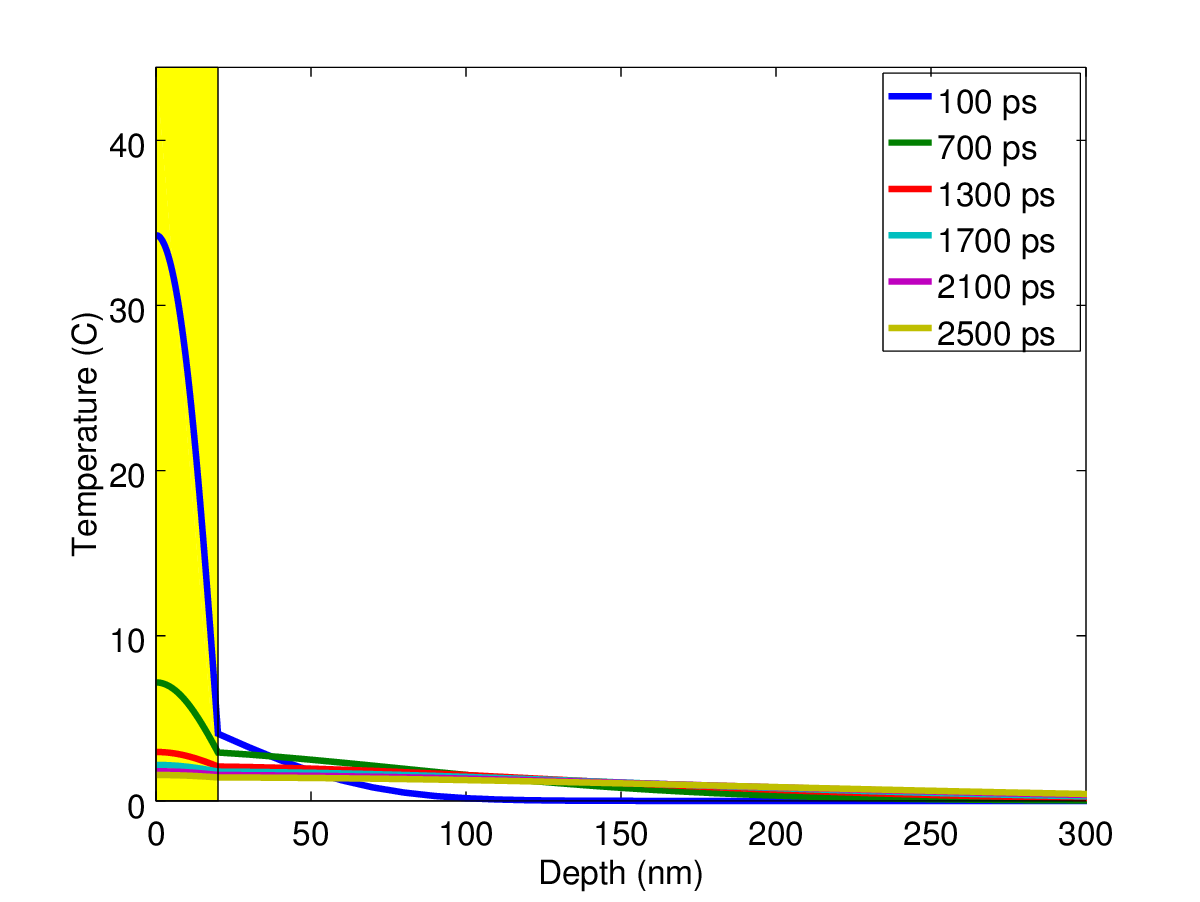
\includegraphics[scale = 0.5]{TempProfile20.png}
\caption{Classical thermal transport result for 20 nm Bi$_2$Se$_3$ on Sapphire  with an absorbed laser fluence of 0.1 mJ/cm$^2$.}
\end{figure}
\begin{figure}[h]
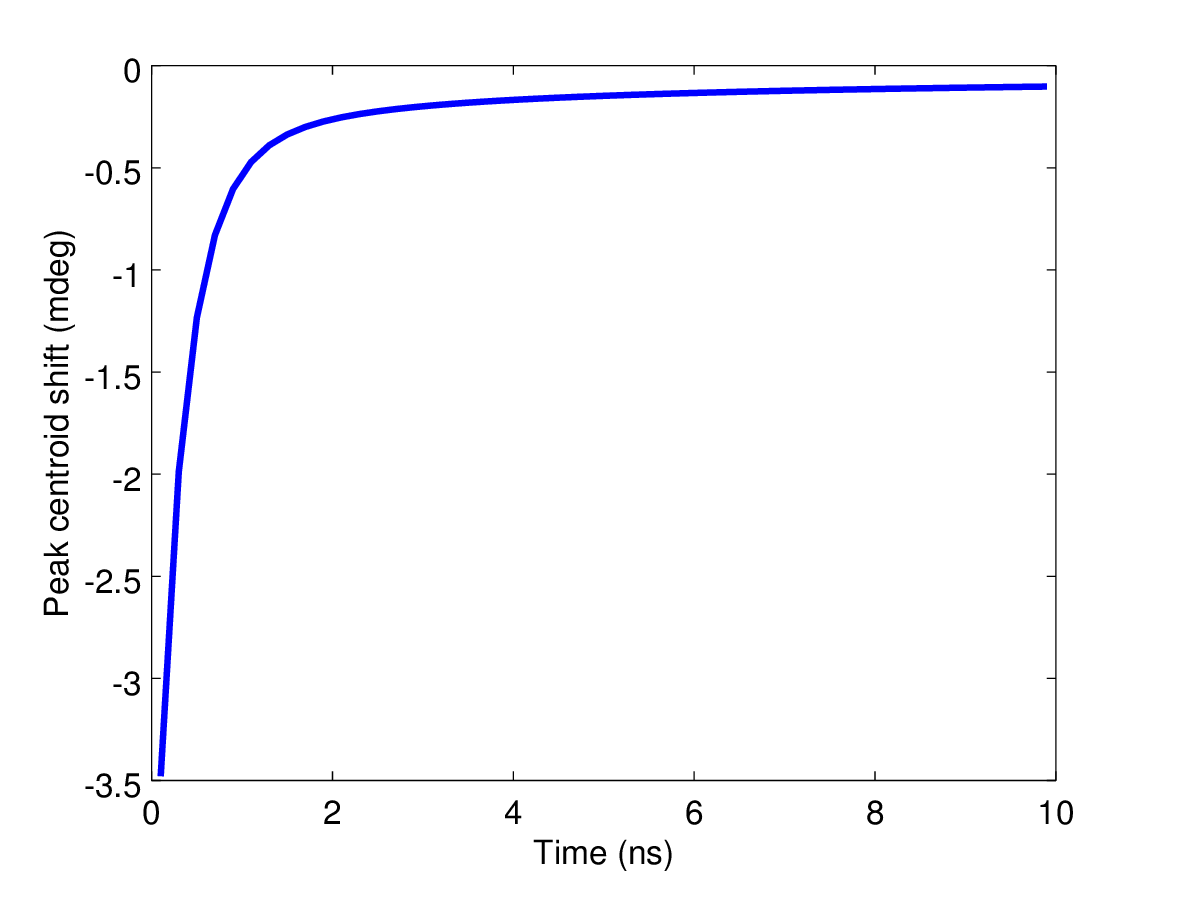
\includegraphics[scale = 0.5]{CentroidShift20.png}
\caption{TRXD calculations corresponding to classical thermal transport result for 20 nm Bi$_2$Se$_3$ on Sapphire.  This is a kinematic diffraction calculation, and the centroid shift is measured relative to before the laser excites the sample.}
\end{figure}
\newpage
\subsubsection{150 nm film}
A 150 nm thick film gives a temperature rise of 5.1 K.  After 9.9 ns, the average film temperature rise is only 2.5 deg C. The maximum bulk temperature rise is only 0.5 deg C.
\begin{figure}[h]
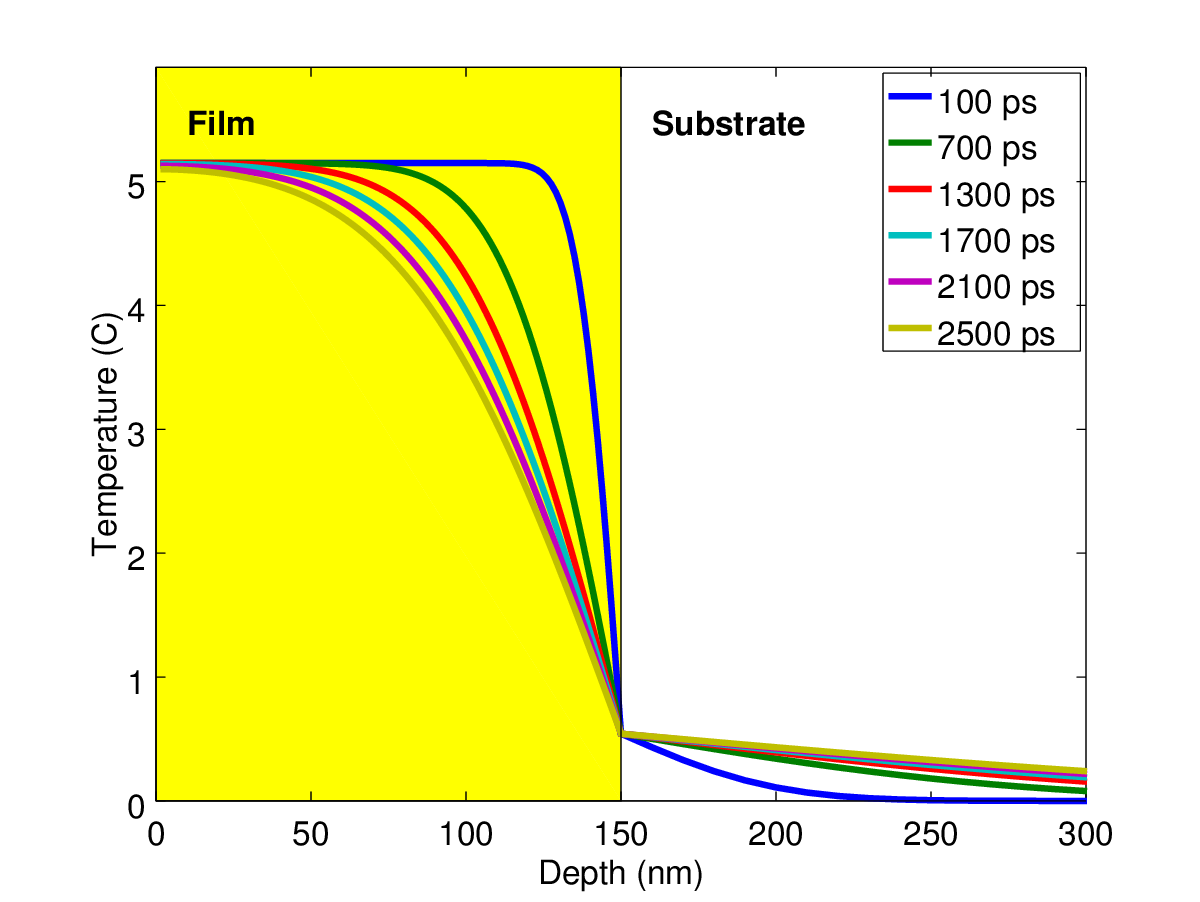
\includegraphics[scale = 0.55]{TempProfile150.png}
\caption{Classical thermal transport result for 150 nm Bi$_2$Se$_3$ on Sapphire with an absorbed laser fluence of 0.1 mJ/cm$^2$.}
\end{figure}
\begin{figure}[h]
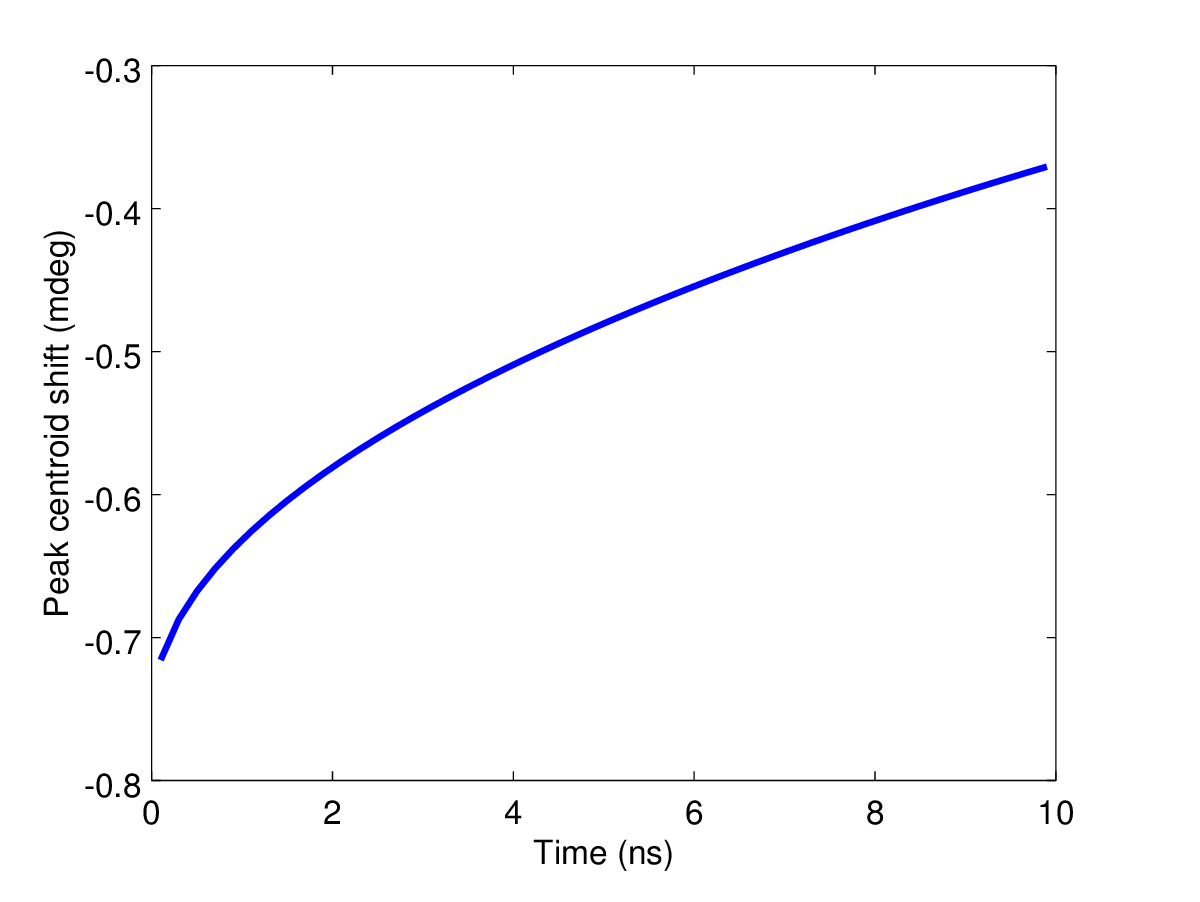
\includegraphics[scale = 0.55]{CentroidShift150.png}
\caption{TRXD calculations corresponding to classical thermal transport result for 150 nm Bi$_2$Se$_3$ on Sapphire.  This is a kinematic diffraction calculation, and the centroid shift is measured relative to before the laser excites the sample.}
\end{figure}

\newpage


\section*{Appendix: Parameters}

\begin{table}[h]
\begin{centering}
\begin{tabular}{c | c | c | c}
parameter  & Bi$_2$Se$_3$ & Sapphire & unit \\
\hline
Specific Heat & 189.83 & 761.00 & J/(kg K) \\
Density & 6820 & 3980 & kg/m$^3$ \\
Thermal Conductivity & 0.75 & 23.1 & W/(m K) \\
Thermal Expansion & 1.9 $\times 10^{-5}$ & - & 1/K \\
Bragg Angle & 7.7 & - & degrees \\
\end{tabular} 
\caption{Material properties used in these calculations. }
\label{table:sign_conventions}
\end{centering}
\end{table}

\pagebreak
\section*{Appendix: Code}

The most recent and up to date code should be obtained from \url{https://github.com/elandahl/Bi2Se3_thermal}.  This code listing is for reference only. 

\verbatiminput{Bi2Se3_thermal.m}

\end{document}
